\documentclass[12pt]{article}

%**********************************************
%* Add additional packages as needed

\usepackage{acronym}
\usepackage{url,amsmath,setspace,amssymb}
\usepackage{listings}
\usepackage{hyperref}
\usepackage{booktabs}

\usepackage{tcolorbox}
\usepackage{tikz}
\usepackage{xcolor}


\usepackage{color}
\def\R{\color{red}}
\def\B{\color{blue}}

\usepackage{listings}
\usepackage{caption}


%**********************************************
%* Please replace this with your name and your AAU student number
\newcommand{\studentname}{Magnus Offermanns}
\newcommand{\studentnumber}{01360639}



%**********************************************
%* Some more or less useful stuff, add custom stuff as needed

\lstnewenvironment{myalgorithm}[1][] %defines the algorithm listing environment
{
   % \captionsetup{labelformat=algocaption,labelsep=colon}
    \lstset{ %this is the stype
        mathescape=true,
        frame=none,
        numbers=none,
        basicstyle=\normalsize,
        keywordstyle=\color{black}\bfseries\em,
        keywords={,input, output, return, datatype, function, in, if, else, foreach, while, begin, end, },
        numbers=left,
        xleftmargin=.04\textwidth,
        #1 % this is to add specific settings to an usage of this environment (for instance, the caption and referable label)
    }
}
{}


\newtcolorbox{alert}[1]{
colback=red!5!white, colframe=red!75!white,fonttitle=\bfseries, title = #1}

\newtcolorbox{commentbox}[1]{
colback=black!5!white, colframe=black!75!white,fonttitle=\bfseries, title = #1}


%**********************************************
%* Leave the page configuration as is
\setlength{\oddsidemargin}{.25in}
\setlength{\evensidemargin}{.25in}
\setlength{\textwidth}{6.25in}
\setlength{\topmargin}{-0.4in}
\setlength{\textheight}{8.5in}

\newcommand{\heading}[5]{
\renewcommand{\thepage}{#1-\arabic{page}}
\noindent
\begin{center}
	\framebox[\textwidth]{
	\begin{minipage}{0.9\textwidth} \onehalfspacing
	{\bf 650.025 -- \unitname} \hfill #2

	{\centering \Large #5

	}\medskip
	{#3 \hfill #4}
	\end{minipage}
}
\end{center}
}

\newcommand{\unitname}{Machine Learning and Deep Learning}
\newcommand{\maxpages}{10}
\newcommand{\handout}[3]{\heading{#1}{#2}{\studentname}{\studentnumber}{#3}}

%**********************************************
%* The document starts here
\begin{document}

\handout{\maxpages}{Winter Term, 2021/22}{Bio-activity estimation}

\section{Code repository}
The code can be found in the repository: \href{https://github.com/MagnusOffermanns/beta-lactamase}{MagnusOffermanns/beta-lactamase}

\section*{Outline and Motivation}
% TODO: find the right kind of beta lactamase in the dataset
Drug research is often supported by computational analysis. One good indicator if a drug is effective at the right place is to monitor its bio activity towards the targeted human protein. This bio activity can be determined experimentally in laboratories, which is costly. To reduce the experimental workload, a filtering in which we eliminate molecules that are unlikely to match to the proteins is therefore very valuable. Therefore we want to implement a machine-learning algorithms to predict the bio-activity of molecules to wards a protein that is called \textit{beta-lactamase}.\\\\
As features we use descriptors calculated from the \textit{Mol} representation of the molecules which is a standard class in the \href{https://www.rdkit.org/docs/source/rdkit.Chem.html}{Rdkit.Chem}. Therefore we use  \href{https://github.com/mordred-descriptor/mordred}{Mordred} a molecular descriptor calculator which calculates about 1600 descriptors calculated from the 2D and 3D representation of the molecules.\\  
We implemented three estimation algorithms: A random forest, a multi-layer-perceptron both using \href{https://scikit-learn.org/stable/}{scikit-learn} and a deep neural-net using \href{https://keras.io/}{Keras}. Lastly we compare the approaches and point out difficulties in training and their consequences in the estimation performance.\\\\
%
In section \ref{sec:Dataset} we describe the Dataset, it's structure and its complexities. In section \ref{sec:Descriptors} we describe the descriptors calculated with \href{https://github.com/mordred-descriptor/mordred}{Mordred} and their meaning and how low quality features were eliminated. Then we give an overview over the code in section \ref{sec:code}. In section \ref{sec:architectures} we discuss the architectures of the different classifiers. In the evaluation section \ref{sec:Evaluation} we compare the performances of the different approaches and discuss how the estimation accuracy could be improved upon. Lastly in section \ref{sec:Conclusio} we discuss the learnings of this project and steps that could have been implemented with additional time at hand.


\section{Dataset}\label{sec:Dataset}
The dataset was compiled by a Data-science Youtuber and was compiled from data of the bio-informatics database \href{https://www.ebi.ac.uk/chembl/}{ChEMBL}. In table \ref{tab:dataset} one can see a representative part of the dataset consisting of 8 Molecules. The first column named \textit{molecule\_chembl\_id} is a unique identifier of each molecule. The second column called \textit{canonical\_smiles} is a string representation of the structural makeup of the molecule and common in many bio-informatics application. In table \ref{tab:dataset} we only show the first two characters of the representation. The third column \textit{standard\_relation} and \textit{standard\_value} are describing a
the bio-activity value. While the column \textit{standard\_value} describes the numerical value the column \textit{standard\_relation} refers to a feature of the machine the value was measured with. If the measured value is bigger than the measurable range of the machine, the maximum value possible is inserted and the value of the column is set to '$>$' to indicate that an overflow over the measuring range occurred. This can be seen in row Nr. six. Hence the value displayed can be far higher than the displayed value. The two following columns \textit{standard\_units} and \textit{standard\_type} are describing the unit and the measuring procedure and are not relevant for the evaluation. The following column \textit{pchembl\_value} is a derived value and a logarithmic representation of the column \textit{standard\_value} calculated by formula \ref{eqn:pchembl}. It is used to generate the binary labels.

\begin{equation}
\label{eqn:pchembl}
\text{pchembl\_value}=-log(\text{standard\_value})
\end{equation}

 If the value is bigger than 6 we consider the element as bio-active (True) otherwise as bio-inactive (False). We have about 20 \% active molecules and 80\% inactive molecules which makes the dataset strongly dis-balanced. Measures to make the dataset more balanced are described in section \ref{sec:Dataset:pre-processing}. The column \textit{target\_pref\_name} is determining the target protein the molecule wants to bind to. As there are different kinds of beta-lactamase (here visualized as beta-lactamase-1 till beta-lactamase-4) we will only use the molecules that bind to a specific form of beta-lactamase. The last column \textit{binary} is the output term and determines if we consider the molecule as active or inactive.\\ In the following chapter we will discuss how we filtered and pre-processed the data to create viable datasets. 
%
\begin{table}[t]
\centering
\begin{tabular}{lllrllrll}
\toprule
CHEMBL606647 &  CO & = &  25000.0 & nM & IC50 & 4.60 & Beta-lactamase-1  & False \\
CHEMBL277857 &  CC & = &  96200.0 & nM & IC50 & 4.02 & Beta-lactamase-1  & False \\
 CHEMBL84953 &  CC & = & 100000.0 & nM & IC50 & 4.00 & Beta-lactamase-2  & False \\
CHEMBL177772 &  C[ & = &   1600.0 & nM & IC50 & 5.80 & Beta-lactamase-1  & False \\
CHEMBL175189 &  C[ & = &    120.0 & nM & IC50 & 6.92 & Beta-lactamase-2  &  True \\
  CHEMBL1239 & CC & $>$ &  90000.0 & nM & IC50 & 4.05 & Beta-lactamase-1  & False \\
    CHEMBL91 & CO & = &  40000.0 & nM & IC50 & 4.40 & Beta-lactamase-3  & False \\
   CHEMBL808 & C[ & = &  25000.0 & nM & IC50 & 4.60 & Beta-lactamase-1 & False \\
\bottomrule
\end{tabular}

\caption{Snapshot of the Dataset}
\label{tab:dataset}
\end{table}
%
%
\subsection{Descriptors}\label{sec:Descriptors}
The descriptors used for classification were calculated using the  \href{https://github.com/mordred-descriptor/mordred}{Mordred} \cite{mordredpaper} library. It can calculate upto 1600 2D and 3D descriptors. These are describing certain properties of the molecule for example the number of acids, the number of carbon atoms or the size of the entire Molecule. As many 3D descriptors return NaN values, we decided to focus on 2D descriptors. There are 198 descriptors with int datatype, 467 with float datatype and lastly 2 descriptors who are boolean. In our model we only work with numerical features, as it is not clear which integer features are categorical and which are not, due to a lack of information what the features actually mean. Therefore we eliminate the boolean features and the integer features in order to prevent bad data from lowering the estimation quality. With further background knowledge on descriptors they could be included into a future model by transforming them into a single feature space.\\\\
%
Also the remaining data is not optimal, we encounter big value differences in certain descriptors. Further we are not aware which descriptors actually contain information if a molecule is biologically active. We can assume that some of the descriptors do not contain any information and are only adding noise.\\\\
%
Summing up we can say that the data is non optimal, due to the dis-balance of the dataset and the lack of information on the descriptors. Additional filtering is necessary and will described in the next chapter.  
\subsection{Pre-processing and creation of the dataset.}
\label{sec:Dataset:pre-processing}
%pre-descriptor filtering
%molecules where the expriment did not target beta-lactamase-1
%molecules where the measured value is the maximum of the laboratory machine.
%combination of molecules where we have multiple measurments
%descriptor filtering
%Descriptors that produce only missing values (occurs often with 3D-Descriptors)
% Descriptors that produce missing values in multiple Molecules
% possible filters: where minimum and maximum value is to far apart -> logarithmic  

We want to split the pre-processing into three parts. First the filtering of molecules necessary before the calculation of the descriptors and the calculation after the calculation of the descriptors. Lastly we have to choose the used descriptors.\\
First we eliminate molecules that do not target the beta-lactamase AmpC but another form of beta-lactamase.\\
%
In the next step we eliminate molecules where the measured value is above the measuring range of the laboratory equipment. This is the case when there is a '$>$' in the entry of the column \textit{standard\_relation}.\\
%
Lastly we combine measurements of the same molecule. We calculate the mean and the standard deviation of each molecule group eliminating molecules that have a \textit{pchembl\_value} more than two standard deviations away from the mean. We re-calculate the mean after discarding irregular values and keep one molecule with the \textit{pchembl\_value} equal to the calculated mean.\\\\
%
In the next step we calculate descriptors and choose which descriptors are used for the fitting of the model. First we eliminate all descriptors that produce NaNs as a result. This are mainly 3D-descriptors. Then we filter descriptors that have more NaNs than a certain threshold. About 3000 NaNs in dataset of 65000 molecules was chosen as threshold, as most descriptors fail to calculate values on the same 2500 molecules.\\\\
%
Afterwards we eliminate all molecules that have NaNs as descriptors. With this filtering about 61000 molecules with 900 descriptors remain.\\\\
%
I actively decided against interpolation of NaN values as we have not enough information about the individual descriptors and the diversity of the molecules. Further we face in some descriptors strongly varying magnitudes(i.e. a big range of values for instance between $10^-3$ to $10^6$). Therefore a logarithmic conversion could be of value but as this only concerns individual descriptors, we omitted this step.\\\\ 
%
Then, due to the class imbalance (20\% active, 80 \% inactive) of the original dataset, the dataset is oversampled. This occurs by splitting the original dataset into two datasets one containing  the active molecules and one containing all inactive molecules. Then we assemble the new datasets out of $n$ times all active molecules (which is about 20 \% of the whole dataset) and a random sample of inactive molecules equal to the number of active molecules. I choose n to be 2. Resulting we have a dataset with 50\%/50\% active/inactive molecule distribution. The size of the dataset is about 45000 molecules.\\\\
%logarithmic for descriptors with high differences, NaN filling
In the next chapter we will describe the structure of the code and it's execution.
%
%
\section{Code overview}\label{sec:code}
In this section we give an overview over the individual options when executing this program. The program can be executed with the following command while \texttt{option} stands for one of the later explained options.
%
\begin{center}
\begin{tabular}{c}
\begin{lstlisting}[language=bash]
python main.py option
\end{lstlisting}
\end{tabular}
\end{center}
%
The first four options are concerning dataset creation from the raw data and filtering and need to be executed after each other. Those are : \texttt{prepare\_dataset},\texttt{calculate\_fingerprints}, \texttt{filter\_descriptors} and \texttt{create\_train\_validate\_test}.\\
The three options \texttt{random-forest},\texttt{multi-layer-perceptron} and \texttt{keras-deep-model} are starting the training of the three models. We will describe them more detailed in section \ref{sec:architectures:random forest}, \ref{sec:architectures:Multi-layer-perceptron} and \ref{sec:architectures:Keras-deep-model}.\\
The last option we implemented was the option \texttt{descriptor\_stats} which calculates and outputs certain statistics as datatype, max value,min value, mean value and standard deviation. Lastly the option \texttt{evaluate} calculates the confusion matrices and scores of each model.

\subsection{download}
When executing \texttt{python main.py download} the zib-file containing the dataset is downloaded from Github and is unziped into 137 zib files. 

\subsection{prepare\_dataset}
When executing \texttt{python main.py prepare\_dataset} we first read in the previously downloaded CSV files and convert them to a pandas DataFrame. Then we remove molecules without a smiles representation, pchembl value and, molecules that have a different target than \textit{'Beta-lactamase AmpC'}. Furthermore we eliminate molecules that returned pchmbl values greater than the measuring range of the machine. Lastly we combine molecules that occur double in the dataset following the description of section \ref{sec:Dataset:pre-processing}.\\ Then we create an output column for binary and class descriptors based on the \textit{'pchembl\_value'} column.\\ Lastly we calculate the mol notation needed for the descriptor calculation from the already existent \textit{smiles} notation.\\\\
The resulting dataset is saved as a file in \texttt{./Data/dataset/cleaned\_dataset.pkl}
 
\subsection{calculate\_fingerprints}
When executing \texttt{python main.py calculate\_fingerprints} we use the mordred library \cite{mordredgit,mordred_paper} to calculate 2-D descriptors from the previously calculated mol representation. The result are about 1600 descriptors that are filtered and refined when executing \texttt{filter\_descriptors}.\\
The calculation takes on a laptop about 3 hours and takes great amounts of RAM. Therefore, it might comes to stops if not enough memory is present. In that case the calculation has to be restarted. To not recalculate already calculated descriptors one can adapt the running variable of the for loop in \texttt{Data\_functions.calculate\_descriptors} to start not at 0 but at the wanted number. 

\subsection{filter\_descriptors}
When executing \texttt{python main.py filter\_descriptors} one can filter descriptors based on the number of NaN entries and the datatype. Then all molecules that have a NaN entry in one of their descriptors are filtered and one complete dataset is created.\\
Which descriptors are filtered can easily be adapted by adding functions to the \texttt{FilterClass}.

\subsection{create\_train\_validate\_test}
When executing \texttt{python main.py create\_train\_validate\_test} three steps are done. First, due to the class imbalance of the original dataset, the dataset is oversampled. This occurs by splitting the original dataset into two datasets one containing the active molecules and one containing all inactive molecules. Then we assemble the new datasets out of $n$ times all active molecules (which is about 20 \% of the whole dataset) and a random sample of inactive molecules equal to the number of active molecules. I choose n to be 2. Resulting we have a dataset with 50\%/50\% active/inactive molecule distribution. The size of the dataset is about 45000 molecules.\\\\
%
Secondly the dataset is split up in three parts,train with 65\% of datasets , validate with 15\% of the datasets and test with the remaining 20 \%.  This is inline with rule of thumbs and was adapted experimentally during development.\\\\
%
Lastly the dataset is normalized using scikit-learns' StandardScaler.

\subsection{random-forest}
When executing \texttt{python main.py random-forest}, the model that is trained is the scikit-learns Random forest classifier \cite{RandomForest}. Instead of running it on the standard parameters I doubled the number of trees in the estimated random forest.

\subsection{multi-layer-perceptron}
When executing \texttt{python main.py multi-layer-perceptron} the trained model is scikit-learns class \texttt{MLPClassifier} that implements a multi-layer-perceptron using backpropagation \cite{MLPclassifier}.The algorithm used is 'adam'. The chosen architecture will be described further in chapter \ref{sec:architectures}.

\subsection{keras-deep-model}
When executing \texttt{python main.py keras-deep-model} we train a defined keras Sequential-model running the adam algorithm. The architecture will be described further in chapter \ref{sec:architectures}. 

\subsection{descriptor\_stats}
When executing the command \texttt{python main.py descriptor\_stats} analysis of the individual descriptors are printed. This includes the max and min value, mean and standard deviation, the number of unique values the number of NaNs, the most common value and the frequency of the most common value. In listing \ref{descriptor_stats} one can see an example output of a descriptor. I decided against \texttt{Dataframe.Describe} as mordred introduces mordred objects into the dataframe and hindered the use of standard functions. 

\begin{lstlisting}[language=bash,caption={Statistics about the ETA\_espilon\_5 descriptor},label=descriptor_stats]
Name: ETA_epsilon_5  
max : 1.229762      min: 0.652381
mean: 0.832055 std_dev: 0.045008
uniq: 0015356 num_nan: 0002164
com : 0.800000 freq: 0000254 
type: <class 'float'> | nr: 61740  
\end{lstlisting}

\subsection{evaluate}
When executing \texttt{python main.py evaluate} all model scores are calculated and confusion matrices are displayed. Additionally loss and accuracy curves are displayed.

\section{Architectures}
\label{sec:architectures}
In this chapter we describe the architectures of the individual models. In section \ref{sec:architectures:random forest} we describe the architecture of the random forest, in section \ref{sec:architectures:Multi-layer-perceptron} we describe the architecture of the scikit-learn Multi-layer-perceptron and lastly in section \ref{sec:architectures:Keras-deep-model} we describe the architecture of the defined model in keras.

\subsection{Random Forest}
\label{sec:architectures:random forest}
We used the function \texttt{RandomForestClassifier} provided by scikit learn. As our Dataset is complex we increased the number of trees in the forest to 200. With bigger sizes we had problems with the memory. Therefore the parameter of \texttt{max\_depth} could be used, but after experiments we were not able to see an improvement of the performance when reducing the depth of the trees for having more trees.

\subsection{Multi-layer-perceptron}
\label{sec:architectures:Multi-layer-perceptron}
The multi-layer-perceptron we implemented had additionally to the input and output layer two hidden layers with the size of 400 each. We followed the advice of Sandhya Krishnans \cite{NumNeurons} article in which she cites 3 rules from literature \cite{Neunets2}:
\begin{itemize}
\item The number of hidden neurons should be between the size of the input layer and the size of the output layer.
\item The number of hidden neurons should be 2/3 the size of the input layer, plus the size of the output layer.
\item The number of hidden neurons should be less than twice the size of the input layer.
\end{itemize}

As we have about 400 descriptors we almost fulfill all three rules.
\subsection{Keras deep neural network}
\label{sec:architectures:Keras-deep-model}
As described the deep neural network built with keras did not have good performance. The models seem to be mainly guessing and the best accuracy of all architectures was 57\% achieved by the $\textit{baseline simmilar to MLPC}$ model(See table \ref{tab:architectures} for reference).
In every architecture the activation function used was either Relu, in the last layer we used sigmoid as activation function in order to receive a probability output between 0 and 1 which can be converted to the two classes easily.\\
I implemented three main architectures, first a baseline to compare to the scikit-learn MLPC-classifier that has 400 neurons in two layers. Second I implemented a small network with two layers with 60 and 30 neurons to see how well a network could perform without over-fitting. Lastly I implemented a network with 5 layers starting with 400 neurons and from there halving the number of neurons. I added also a dropout-layer to prevent over-fitting. For reference the architectures are listed in table \ref{tab:architectures}.
 
\begin{table}[t]
\centering
\begin{tabular}{lll}
\hline
\multicolumn{1}{|l|}{Baseline simmilar to MLPC} & \multicolumn{1}{l|}{Small} & \multicolumn{1}{l|}{Deep} \\ \hline
dense(400,act=relu)                             & dense(60,act=relu)         & dense(400,act=relu)       \\
dense(400,act=relu)                             & dense(30,act=relu)         & dropout(0.5,act=relu)     \\
dense(1,act=sigm)                               & dense(1,act=sigm)          & dense(200,act=relu)       \\
                                                &                            & dense(100,act=relu)       \\
                                                &                            & dense(50,act=relu)        \\
                                                &                            & dense(1,act=sigm)        
\end{tabular}
\caption{Snapshot of the Dataset}
\label{tab:architectures}
\end{table}

\section{Evaluation}\label{sec:Evaluation}
Summarizing it can be said that the cleaning and creation of the dataset was definitely the most time intensive and challenging work, due to a lack of experience of both biological data and to the handling of big datasets. The biggest influence on performance had the countering of the class-imbalance of the dataset. Before the oversampling described in section \ref{sec:Dataset:pre-processing} all classifiers learned to give all molecules the inactive flag resulting in a 80 \% accuracy rating (as seen during the presentation).\\
%
Both scikit-learn functions performed very well but due to the oversampling, it can occur that some of the molecules re-appear in training and test set which means that the performance of the classifiers on entirely unbiased data might be slightly worse. The designed keras-deep model did not perform well and I guess that I still have somewhere an error in the design.\\ The accuracy scores of the models are: Random forest classifier: 89.04\%, MLP-classifier: 83.58 \% and for the keras-deep model: 56.35\% and can be seen in the figures \ref{fig:conf_m1},]\ref{fig:conf_m2} and \ref{fig:conf_m3}.

\begin{figure}[!htb]
\minipage{0.32\textwidth}
  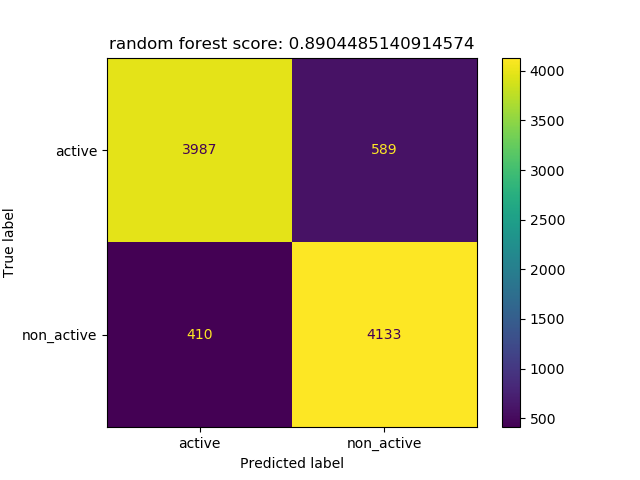
\includegraphics[width=\linewidth]{./figures/random_forest_confusion_matrix.png}
  \caption{Random Forest}\label{fig:conf_m1}
\endminipage\hfill
\minipage{0.32\textwidth}
  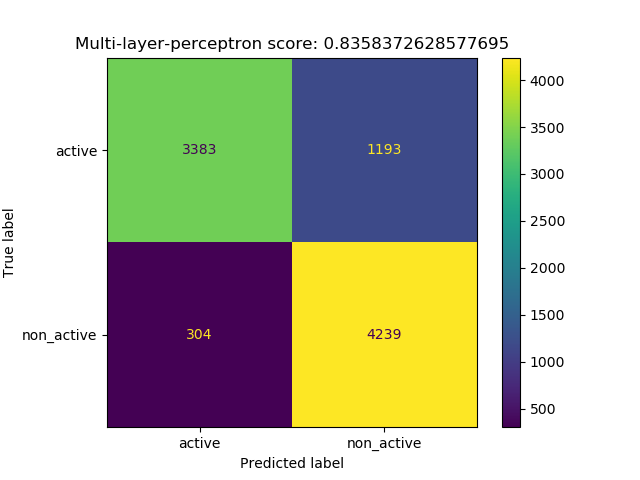
\includegraphics[width=\linewidth]{./figures/Mulit-layer-perceptron_confusion_matrix.png}
  \caption{MLP-classifier}\label{fig:conf_m2}
\endminipage\hfill
\minipage{0.32\textwidth}%
  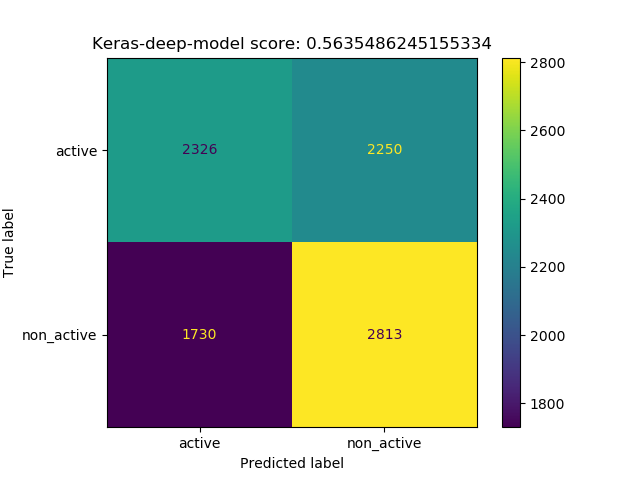
\includegraphics[width=\linewidth]{./figures/keras-deep-model-confusion_matrix.png}
  \caption{Keras-deep-model}\label{fig:conf_m3}
\endminipage
\end{figure}

The most surprising observation in line with the paper \cite{robinson2020} that was also cited in the project proposal is that also less complex classifiers like the Random-forest-classifier can perform very well. My personal guess is that the neural-networks could outperform the RF-classifier, but it needs considerably more fine-tunig. This performance needs to be taken with a grain of salt, as we are reusing the active molecules. Therefore we can imagine that the performance on a totally unrelated dataset would be smaller.

\begin{figure}[!htb]
\minipage{0.32\textwidth}
  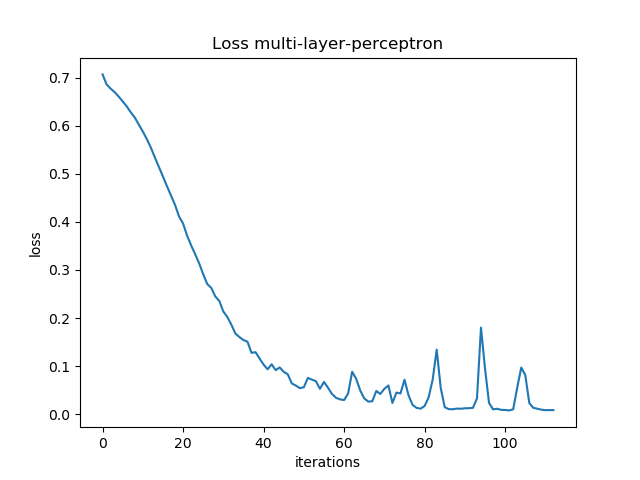
\includegraphics[width=\linewidth]{./figures/multy_layer_perceptron_loss_curve.png}
  \caption{Loss MLP}\label{fig:loss_MLP}
\endminipage\hfill
\minipage{0.32\textwidth}
  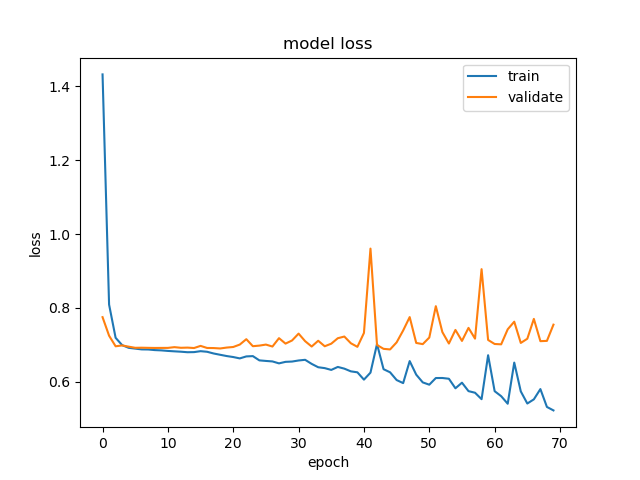
\includegraphics[width=\linewidth]{./figures/keras-deep-model-loss-curve.png}
  \caption{Loss keras-deep-model}\label{fig:loss_keras}
\endminipage\hfill
\minipage{0.32\textwidth}%
  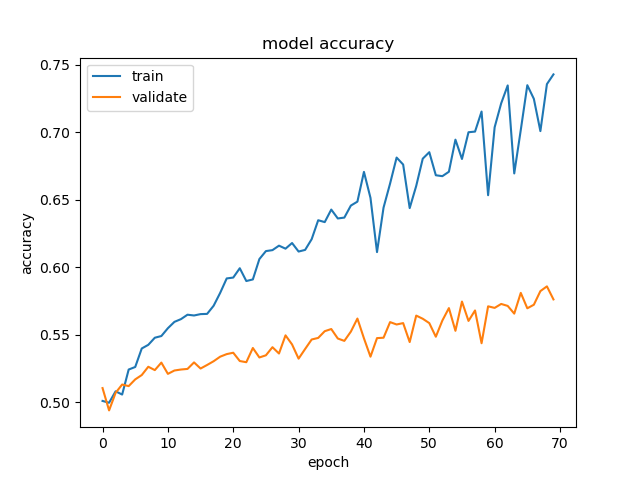
\includegraphics[width=\linewidth]{./figures/keras-deep-model-accuracy-curve.png}
  \caption{Accuracy keras-deep-model}\label{fig:accuracy_keras}
\endminipage
\end{figure}

The loss curve of the Multilayer-perceptron in figure \ref{fig:loss_MLP} looks very similar to a optimal loss curve. It starts at about 0.7 and finishes at 0.06. This is also  reflected in the performance. In comparison, the loss curve of the keras-deep-model \ref{fig:loss_keras} is starting very high and is stopping at about 0.6 which is not low enough for a good estimation. Additionally the curve decreases at the start strongly. To counter this I lowered the learning rate but, the form of the curve changed little and the performance worsened.\\In figure \ref{fig:accuracy_keras} one can see the accuracy of the estimation between training and validation set. From about epoch 5 we slowly over-kfit which is in line with the loss curve. The accuracy on the training set in the end of the computation is bigger than 75 \% while it is well below 60\% in the validation set. This  is also in-line with the bad performance of the classifier on the test-set.
 
\section{Conclusion and Future-work}\label{sec:Conclusio}
Summarizing it can be said that the random-forest algorithm outperforms both neural nets. This is in line with the literature \cite{robinson2020}, but still surprising.
%
In the future the dataset needs to be cleaned even more, and more information about the individual features need to be collected to use the data efficiently.
%
Further, the setup of the keras-deep-model needs to be restructured and possible errors should be eliminated.

\bibliographystyle{IEEEtran}
\bibliography{bibliography}


\end{document}



